%%%%%%%%%%%%%%%%%%%%%%%%%%%%%%%%%%%%%%%%%%%%%%%%%%%%%%%
% A template for Wiley article submissions developed by 
% Overleaf for the Overleaf-Wiley pilot which ran 
% during 2017 and 2018.
% 
% This template is no longer supported, but is provided
% for historical reference. Last updated January 2019.
%
% Please note that whilst this template provides a 
% preview of the typeset manuscript for submission, it 
% will not necessarily be the final publication layout.
%
% Document class options:
% =======================
% blind: Anonymise all author, affiliation, correspondence
%        and funding information.
%
% lineno: Adds line numbers.
%
% serif: Sets the body font to be serif. 
%
% twocolumn: Sets the body text in two-column layout. 
% 
% num-refs: Uses numerical citation and references style 
%           (Vancouver-authoryear).
%
% alpha-refs: Uses author-year citation and references style
%             (rss).
%
% Using other bibliography styles:
% =======================
%
% To specify a different bibiography style
%
% 1) Do not use either num-refs or alpha-refs in documentclass.
% 2) Load natbib package with the options set as needed.
% 3) Use the \bibliographystyle command to specify the style
% 
% Included NJD styles are: 
%   WileyNJD-ACS
%   WileyNJD-AMA
%   WileyNJD-AMS
%   WileyNJD-APA
%   WileyNJD-Harvard
%   WileyNJD-VANCOUVER
%
% or you may upload an alternative .bst file 
% (if requested by the journal).
%
% Examples:
% =======================
%% Example: Using numerical, sort-by-authors citations.
\documentclass[num-refs]{wiley-article}

%% Example: Using author-year citations and anonymising submission
% \documentclass[blind,alpha-refs]{wiley-article}

%% Example: Using unsrtnat for numerical, in-sequence citations
% \documentclass{wiley-article}
% \usepackage[numbers]{natbib}
% \bibliographystyle{unsrtnat}

%% Example: Using WileyNJD-AMA reference style and superscript
%%          citations, two-column and serif fonts for AIChE
% \documentclass[serif,twocolumn,lineno]{wiley-article}
% \usepackage[super]{natbib}
% \bibliographystyle{WileyNJD-AMA}
% \makeatletter
% \renewcommand{\@biblabel}[1]{#1.}
% \makeatother
\usepackage{pifont}
\newcommand{\cmark}{\ding{51}}%
\newcommand{\xmark}{\ding{55}}%
% Add additional packages here if required
\usepackage{siunitx}
\usepackage{algorithm}
\usepackage{algpseudocode}
% Update article type if known
\papertype{Original Article}
% Include section in journal if known, otherwise delete
\paperfield{Journal Section}

\title{Securing Logistics System and Supply Chain using Blockchain}

% List abbreviations here, if any. Please note that it is preferred that abbreviations be defined at the first instance they appear in the text, rather than creating an abbreviations list.
\abbrevs{BTC, Bitcoin; USD, United States Dollar; DLT, Distributed Ledger Technology; LC, Letter of Credit; BL, Bill of Lading.}

% Include full author names and degrees, when required by the journal.
% Use the \authfn to add symbols for additional footnotes and present addresses, if any. Usually start with 1 for notes about author contributions; then continuing with 2 etc if any author has a different present address.
\author[1\authfn{1}]{Ajay Kumar}
\author[1]{Kumar Abhishek}
\author[2,3\authfn{1}]{Pranav Nerurkar}
\author[3]{Sunil Bhirud}

\contrib[\authfn{1}]{Equally contributing authors.}

% Include full affiliation details for all authors
\affil[1]{Dept. of CSE, NIT Patna, Bihar, India}
\affil[2]{Dept. of Data Science, MPSTME, NMIMS, Mumbai, Maharashtra}
\affil[3]{Dept. of CE \& IT, VJTI Mumbai, Maharashtra, India}

\corraddress{Dept. of CSE, NIT Patna, Bihar, India}
\corremail{ajayk.phd18.cs@nitp.ac.in}

\presentadd[\authfn{2}]{Dept. of CSE, NIT Patna, Bihar, India}

\fundinginfo{This work was supported in part by the Raman Charpak Fellowship of the Indo-French Centre for the Promotion of Advanced Research Grant no: IFC/4132/RCF 2019/716.}

% Include the name of the author that should appear in the running header
\runningauthor{Ajay Kumar et al.}

\begin{document}

\begin{frontmatter}
\maketitle

\begin{abstract}
Past international trade practices have been associated with opaque information flows that have hindered traceability and created hurdles in hassle free trade. Blockchain and allied technologies have been investigated as panacea for the problems faced by supply chain and logistics industry. However, previous literature has focused on limited aspects of a typical supply chain such as monitoring assets, securing traceability widely neglecting data integrity and data access. To overcome such drawbacks, the current paper proposes permissioned blockchain with relevant processes and functions to obtain a holistic framework for securing supply chain and logistic operations. The efficacy of the proposed framework were demonstrated on case study. It was found that critical loopholes in a current supply chain can be overcome using the proposed framework. Additionally, several outlines for future research are outlined. 

% Please include a maximum of seven keywords
\keywords{Logistics, Supply Chain, Blockchain, Distributed ledger, Intelligent logistics system,}
\end{abstract}
\end{frontmatter}

\section{Introduction}

Blockchain technologies have the potential to reduce costs in supply chain and logistics by 15\%, contributing to profits and improving the margins of organizations \cite{fu2019operation}. Several startups have taken initiative to provide blockchain integrated supply chain monitoring solutions to the industry \cite{perboli2018blockchain}. Supply chain and logistics are two parts of the same coin. Supply chain focuses on building a cohesive system for delivering value created at a point to the end user. Logistics links the various entities and their defines their roles and responsibilities in the supply chain \cite{perboli2018blockchain, li2020research}. However, the diverse entities present in the supply chain create coordination issues (E.g: exporting from East Africa to Europe requires 200 interactions between 30 or more entities) \cite{chang2020blockchain, hackius2017blockchain}. Excessive paperwork, regulatory compliances are time consuming in case of inter state or inter continental movement of goods. Over 25-50\% of supply chain experts advocate blockchain for reducing transaction costs and improving transparency on supply chain \cite{kolb2019role}. Earlier paper based systems were used which suffered from drawbacks of file management systems. Upon the entry of digitization, due to the databases the issues of having paper-based procedures were overcome to a large extent \cite{paardenkooper2019creating}. 


While digitization solved the problem of atomicity, storage and consistency with the use of database management systems, it could not address the problem of having a centralized trusted third party. In the event of cross border transfer of goods, the number of centralized regulators increases, each with its own compliance mechanism. This escalates the burden on the members of the supply chain. It is estimated that the contribution of supply chain costs in developing and developed countries varies between 8-14\% \cite{li2020research}. Any savings in this scenario shall provide significant value addition to the consumers and industry. High costs are also caused due to the maintenance of the centralized trusted third party. By eliminating the need for the trusted third party, the compliance costs can be reduced. Elimination of the outside trusted third entity was one of the reasons why blockchain was proposed.

Conceived in 2008 by an unknown individual (or a group of individuals) who used a pseudonym "Santoshi Nakamoto", Bitcoin cryptocurrency has since then emerged as the most successful cryptocurrency amongst its peers, reaching an adoption level unrealized by older digital currencies \cite{park2019nodes, FENG201945, WANG201943}. As on $19^{th}$ March 2020, Bitcoin has a market cap of USD\$98,584,789,143 with 18,277,112 bitcoins (BTC's) in circulation each with a value of USD\$5,393.89. Bitcoin differs from its traditional online banking peers by relying on a decentralized consensus scheme for verifying the correctness and authentic nature of currency transfers between users \cite{rahouti2018bitcoin, nakamoto2019bitcoin, AGGARWAL201913}. The decentralized consensus scheme is made possible by an organized collective of nodes in the Bitcoin system known as ``miners". The miners confirm each transaction for authenticity. This increases security in the Bitcoin system and ensures the core philosophy of Bitcoin "Maintain trust in an untrusted environment" without the need for a trusted third party. As rewards, miners collect transaction fees for the transactions that they confirm. Each user in the Bitcoin network has a private key used to sign transactions. Without the private key, no party can transfer funds. The public key cryptographic mechanisms ensure that it is easy to verify the transaction as initiated by a user without need for the user to divulge his private key. Thus Bitcoin ensures integrity and non-repudiation of transactions. Also as Bitcoin users do not disclose their identities, anonymity and privacy are ensured.

\subsection{Contributions}
\begin{itemize}
    \item Explored applicability of blockchain in streamlining the logistic and supply chain
    \item Conducted a systematic study of blockchain and allied techniques 
    \item Proposed a distributed ledger technology based framework for logistic and supply chain operation management
    \item Conducted through comparison of proposed framework with existing payment process in trade
\end{itemize}

\subsection{Novelty}
Similar to financial sector, even in logistics the application of blockchain is needed to provide decentralized decision making, protecting integrity, anonymity and confidentiality of transactions. But few logistic experts are aware of blockchain and pursue implementation \cite{hackius2020translating, hackius2017blockchain}. Hence, the current paper proposes a framework to implement a private blockchain for securing logistics and supply chain operations of organization. 

\subsection{Outline}
Rest of the paper is divided into following sections: Section \ref{litrev} gives the background and state of the art techniques on blockchain, Section \ref{prop} describes the proposed framework, Section \ref{res} gives the results and discussion of the framework and the paper is concluded in Section \ref{conc}.



\section{Related Works} \label{litrev}


 \subsection{Blockchain and allied technologies}

Illustrating the transaction fundamentals of bitcoin transfers, consider that user $i$ wants to transfer $n$ bitcoins to user $j$. Then $i$ will need a bitcoin wallet, which holds all his private keys and the wallet address of $j$ (Figure \ref{bit-transfer}). Also, the transaction is valid only if user $i$ signs it using his cryptographic key. 

\begin{figure}[!h]
\centering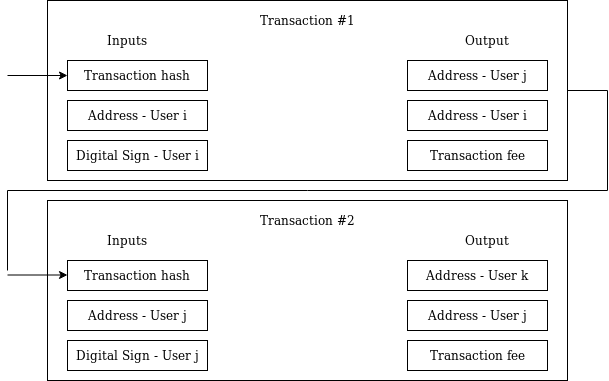
\includegraphics[width=\linewidth]{transactions.png}
\caption{Transfer of bitcoins from user $i$ to $j$ and $j$ to $k$}
\label{bit-transfer}
\end{figure}


Valid transactions are then broadcast over the Bitcoin network, and all miners are informed. Technically, the transaction is not broadcast to all nodes in the Bitcoin network, as a single node can be connected to a maximum 125 (incoming connections=8, outgoing connections=117) other nodes. However, by recursive broadcasts "gossip protocol," a transaction eventually reaches all nodes \cite{park2019nodes, monrat2019survey}. Miners keep all received transactions in their memory pool and combine these transactions to form a "candidate block." Each miner then competes with other miners to add its candidate block to the blockchain. The miner who succeeds gets a reward in BTC's and broadcasts its newly mined block to other miners. Other miners will independently verify the newly mined block before adding it to their blockchain. 


Since Bitcoin's inception in 2009, the initial two years saw slow adoption with hardly 1000 unique addresses and less than 10000 transactions per day \cite{park2019nodes, GHOSH2020102635}. However, as bitcoin became financially significant, there was an exponential growth in transactions from 2012-2016, which also saw the entry of serious users, investors, speculators, and independent mining industries. Before the popularity of bitcoin, the users were mostly crypto-enthusiasts. The change in the profile of Bitcoin's user base was also evident from the increase in the transaction values, fluctuations in BTC price, and volumes of BTC's. This phase also saw the emergence of Ponzi schemes, money laundering, frauds \cite{bohme2015bitcoin}, embezzlements, extortion \cite{reyes2019method} and tax evasion \cite{toyoda2019novel} practices that used the blanket of secrecy afforded by Bitcoin to mislead the audit trail. There emerged a diversity even amongst the miners in terms of geography and size. When Bitcoin was launched, it was feasible for any participant to become a miner, but as the user base increased, mining became competitive and required specialized hardware. Miners prefer large warehouses with access to cheap electricity \cite{alqassem2018anti}. With time, solo miners decreased and gave way to mining pools. 



As the scale and complexity of the Bitcoin network increased, research interest too emerged to allow for its better understanding \cite{rahouti2018bitcoin, toyoda2019novel, alqassem2018anti, lee2019measurements, tschorsch2016bitcoin}. Research has focused on understanding Bitcoins development \cite{tschorsch2016bitcoin}, price fluctuations \cite{saad2019toward}, global statistics \cite{alqassem2018anti}, development of analytical software \cite{park2019nodes}, clustering user identities \cite{toyoda2019novel, pinna2018petri}, surveys on applications, challenges or opportunities \cite{monrat2019survey, yuan2018blockchain} or distributed ledger mechanism of cryptocurrencies \cite{lee2019measurements}. 


There is a complexity of identifying users in the Bitcoin network. In the Bitcoin network, identifying users by wallet addresses (aka accounts, bitcoin addresses, public keys, or other unique identifiers used interchangeably to refer to users' in Bitcoin system) is complicated as these can be generated and discarded multiple times \cite{alqassem2018anti}. There is also no upper limit to the identities a single person can create or any limits on the number of transactions or beneficiaries. These factors significantly enhance the hurdles in analyzing the Bitcoin network. To overcome the hurdle caused by multiple identities of a single user, heuristic clustering is applied to the Bitcoin network. With heuristic clustering, multiple identities of a single user are grouped into a single identity. This strategy is used in several Bitcoin network studies \cite{maesa2019bow, maesa2018graph, maesa2018data, maesa2016uncovering} and has the advantage of reducing the number of entities of the Bitcoin network. 

\subsection{Existing scenario}
Figure \ref{diag-casestudy} gives the description of steps needed to export pharmaceutical products from India. The exporter needs to apply for certificate of origin and no-objection certificate for consignment. Exporter also needs to fill forms for excise and Value Added Tax exemption. Then he loads the consignment to the customs clearing house and obtains a shipping bill which contains information buyer, buyers destination, time needed to ship goods to destination, value of goods, time needed to receive payment from seller, quantity of goods, Unique identifier for type of goods etc. With the shipping bill, the buyer approaches the shipping company to transport the goods. The shipping company provides the buyer with a bill of lading. Upon showing the bill of lading to the exporters bank, the exporter shall receive his payment. The importer issues a letter of credit from his bank in favor of the exporter. The letter of credit is forwarded to the exporters bank and when the terms mentioned in the letter of credit are fulfilled by the exporter, the exporters bank will receive the payment made by the importer. The importers bank transfer the payment of the goods to the exporters bank in return for bill of lading. Once the importers bank receives the bill of lading, the importer is informed. With the bill of lading, the importer can get his shipment from the shipping company subject to customs clearances. The intermediary banks ensure trust between exporter and importer and get convenience fees in exchange.

\begin{figure}[!h]
\centering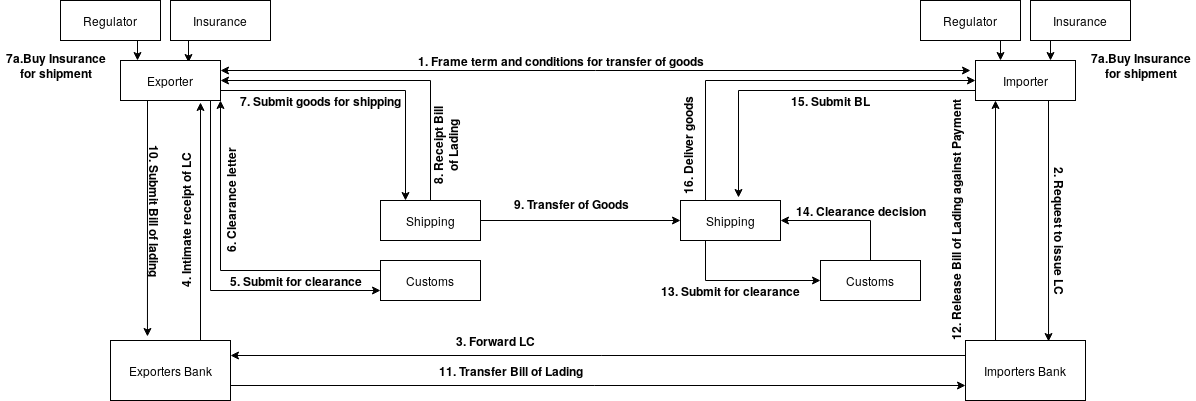
\includegraphics[width=\linewidth]{casestudy.png}
\caption{Export and import procedures - Sequence diagram}
\label{diag-casestudy}
\end{figure}

\subsection{Issues} \label{issues}
\begin{enumerate}
    \item Bill of lading is forged to claim the consignment fee
    \item Letter of credit is forged to defraud exporter
    \item Bill of lading is lost and importer cannot claim the consignment
    \item Bill of lading is stolen and consignment is claimed in place of importer
    \item Bill of lading is stolen and consignment fee is claimed in place of exporter
    \item Consignment is overvalued or undervalued to claim lower tax or higher insurance payout
    \item Convenience fee of intermediary banks may increase costs
\end{enumerate}

\subsection{State of the art}
Figure \ref{diag-ex} gives the flow of interactions between various actors in a typical supply chain \cite{chang2019exploring}. The key intermediary is the bank which acts a trusted third party and channels communication between the various actors. For its mediation, the bank earns its commission or fees. Due to the commission, it is infeasible to have transactions of a minute amount.

\begin{figure}[!h]
\centering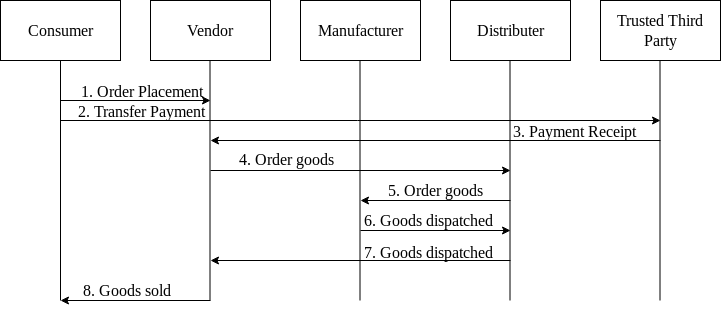
\includegraphics[width=0.8\linewidth]{first.png}
\caption{Existing scenario of logistic and supply chain}
\label{diag-ex}
\end{figure}

K Kuhi \textit{et al.} focused on evaluating efficacy of blockchain based systems for logistics case study  \cite{kuhi2018ensuring}. N Hackius \textit{et al.} \cite{hackius2020translating} interviewed stakeholders in multiple logistic and supply chain organizations to understand how their organizations had adopted blockchain for seamless operations. The authors also highlighted the hype v/s. reality of blockchain in logistic sector. Y Fu \textit{et al.} \cite{fu2019operation} studied the application of blockchain in diminshing the security threats, tracebility, and privacy risks in intelligent logistic systems. X Li \textit{et al.} \cite{li2020research} presented a model for improving the traceability of transactions in blockchain. The aim of the model proposed by them was to overcome issues related to consensus algorithms. A Maiti \textit{et al.} \cite{maiti2019estimating} integrated sensors with and blockchain to create a system for monitoring assets in the supply chain. The proposed framework used blockchain to calculate asset quality in the supply chain. Integrating sensors for farm-to-fork monitoring of agro-based commodities was proposed by M Caro \textit{et al.} \cite{caro2018blockchain}. Though the authors focused only on domestic trade of agro-based commodities, that has a different supply chain compared to international trade of commodities.


From the literature, it is concluded that blockchain is an important technology and can have far reaching impact on logistic sector. However, as there has been limited work proposed in this domain, the current paper proposes a framework for securing logistic and supply chain management using blockchain.

\section{System Framework} \label{prop}
The proposed framework integrates smart contracts with the private, permissioned blockchain to ensure seamless experience for actors involved in a international transaction (see Figure \ref{diag-arch}). The actors participating in such a transaction are listed along with their roles:

\begin{itemize}
    \item Letter of Credit (LC): Documentary agreement of clauses between trading partners that establishes payment if clauses specified are met.
    \item Smart contracts: Programmable protocols capable of self executing if conditions specified while framing the contract are met
    \item Exporter and Importer: Trading partners
    \item Regulator: Statutory body
    \item Issuing bank and Advising bank: Issuing bank issues LC to importer. Advising bank receives bill of lading (BL) from exporter.
\end{itemize}

\begin{figure}[!h]
\centering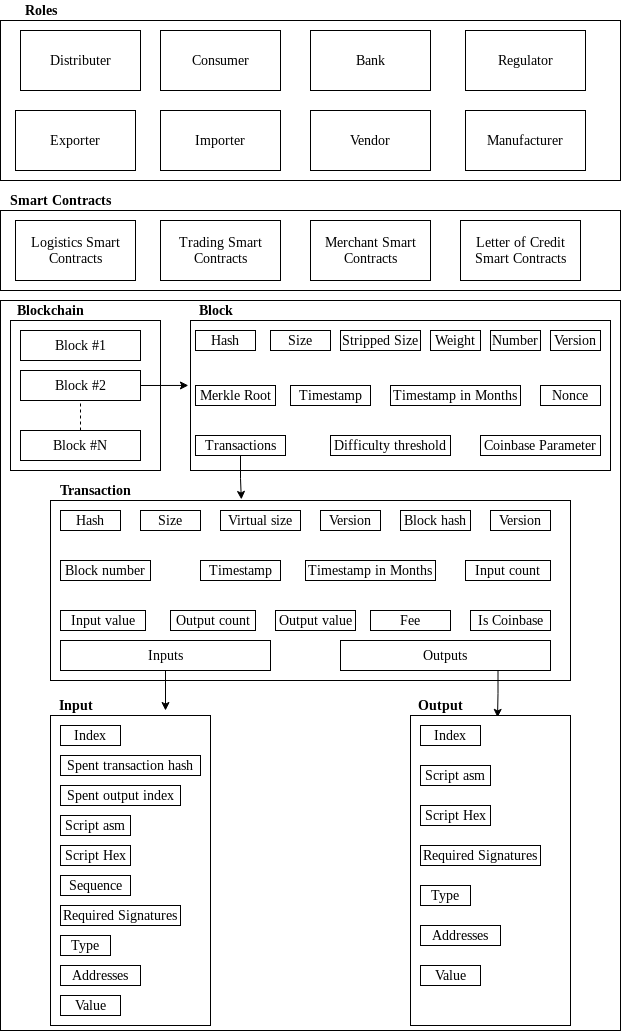
\includegraphics[width=0.6\linewidth]{blockML-logistic.png}
\caption{Architecture of proposed work}
\label{diag-arch}
\end{figure}

The architecture has modules that define roles of various users on the intelligent trading system. It uses smart contracts to avoid centralized decision making. The roles of various smart contracts are explained further. With the use of blockchain, the entire flow of interaction is documented on the distributed ledger. It is tamper-proof and also provides traceability for audit. All entities are identified with wallet addresses and hence the system provides pseudo-anonymity. The role of smart contracts are specified in Figure \ref{diag-sc}, the elimination of intermediaries in the form of issuing and advising bank is the possible with the help of smart contracts.


\begin{figure}[!h]
\centering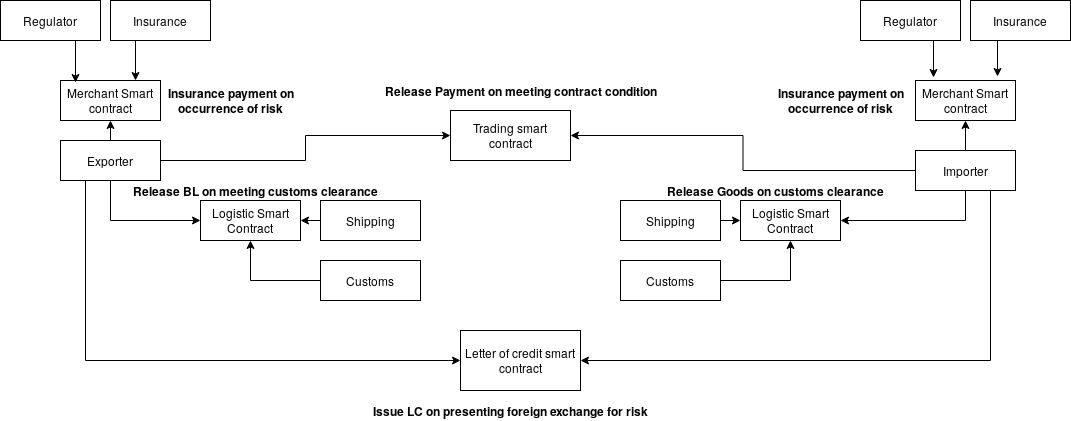
\includegraphics[width=\linewidth]{export.png}
\caption{Interaction and role of smart contracts in proposed framework}
\label{diag-sc}
\end{figure}

\subsection{Steps for designing smart contracts}
\label{algo}

Trading smart contract (see Algorithm \ref{tsc}) is framed between the exporters and importers and records the quality, quantity, delivery date and other clauses decided by the trading entities while making the agreement. If the conditions are met then automatically the payment shall be released to the exporter. 

\begin{algorithm}[!h]
\caption{Designing a trading smart contract}

\begin{algorithmic}[1]
 \State Set initial setting for terms of trade
 \State Set the quality conditions
 \State Set the quantity conditions
 \State Determine the optimal delivery date
 \State Store contract on blockchain
\end{algorithmic}
\label{tsc}
\end{algorithm}

Merchant smart contract (see Algorithm \ref{msc}) is made between the regulator, exporter or importer and the regulator. This ensures that in event of risk the exporter or importer receives automated payment for the insured goods. Conditions specified as per the regulatory framework have to be accepted by insurance company and traders.

\begin{algorithm}[!h]
\caption{Designing a merchant smart contract}
\begin{algorithmic}[1]
 \State Set initial conditions for insurance liability
 \State Set the insurance payout conditions
 \State Store contract on blockchain
\end{algorithmic}
\label{msc}
\end{algorithm}

Logistic smart contract (see Algorithm \ref{lsc} and \ref{lcs1}) is agreed between the customs, shipping company and the exporter. This allows the receipt of the bill of lading and signals to the exporter that the goods may be shipped to destination. Usually the importer needs the bill of lading to collect his goods from the shipping company. 

\begin{algorithm}[!h]
\caption{Designing a logistic smart contract for exporter}
\begin{algorithmic}[1]
 \State Specify customs clearance requirements
 \State Specify conditions of shipping
 \State Store contract on blockchain
 \State Release bill of lading to exporter if conditions met
 \State Confiscate amount of exporter if conditions fail
\end{algorithmic}
\label{lcs1}
\end{algorithm}

\begin{algorithm}[!h]
\caption{Designing a logistic smart contract for importer}
\begin{algorithmic}[1]
 \State Check bill of lading
 \State Check customs clearances for goods
 \State Store contract on blockchain
 \State Issue goods if bill of lading is genuine
 \State Confiscate goods if conditions fail
\end{algorithmic}
\label{lsc}
\end{algorithm}


Letter of credit smart contract (see Algorithm \ref{lcsc}) is made between the exporter and importer. The LC allows the exporter to arrange for cash advances to meet the manufacturing costs and shipping costs.

\begin{algorithm}[!h]
\caption{Designing a Letter of credit smart contract}
\begin{algorithmic}[1]
 \State Submit the credit history and credentials of exporter
 \State Submit the credit history and credentials of importer
 \State Issue LC to importer
 \State Release LC to exporter if credential verified
\end{algorithmic}
\label{lcsc}
\end{algorithm}



\section{Case study and Evaluation} \label{res}
The feasibility and efficacy of the proposed system in Section \ref{prop} is evaluated to check if issues mentioned in Section \ref{issues} are tackled by it.

\begin{enumerate}
    \item Bill of lading is forged to claim the consignment fee: The BL is a transaction between the exporter and the shipping company. The bill will have digital signature of the exporter, importer and shipping company. Once the BL is digitally signed, it will maintain integrity and non-repudiation. No party shall be able to deny their involvement in the contract. Thus, the exporter will have proof of shipment, the shipping company can verify the importer and the both exporter as well as importer can claim damages during shipment or insurance. Exporters bank will be able to verify the identity of the genuine owner of the BL prior to releasing consignment fee. In the proposed system, the Logistic Smart Contract shall release the BL to exporter after clauses of shipping company and customs are met.
    
    \item Letter of credit is forged to defraud exporter: Letter of credit contains digital signatures of importer, exporter, importers and exporters bank. With this verification, integrity and non-repudiation are ensured. LC shall be issued to importers bank to importer after deposit of currency. Finally, the LC Smart contract shall automatically issue to LC to exporter on production of BL.
    
    \item Bill of lading is lost and importer cannot claim the consignment: BL is on the blockchain which makes it available to all users on the blockchain. However, only with the private key of the importer can it be digitally signed. BL can be verified by Shipping company to confirm the recipient.
    
    \item Bill of lading is stolen and consignment is claimed in place of importer: BL is a digital document on the blockchain and hence cannot be stolen or tampered. Without having the private keys of all parties involved (importer, exporter, shipping company) it cannot be claimed. 
    
    \item Bill of lading is stolen and consignment fee is claimed in place of exporter: BL is a digital document on the blockchain and hence cannot be stolen or tampered.
    
    \item Consignment is overvalued or undervalued to claim lower tax or higher insurance payout: Consignment value is based on Merchant Smart contract which is agreed upon by exporter/importer with regulator and insurer. It cannot be changed once agreed and is placed on the blockchain making it tamper-proof.
    
    \item Convenience fee of intermediary banks may increase costs: Intermediary are miners that verify transactions and get a fee for their work. Fees are minimal as verification process is automated.
\end{enumerate}

Data integrity (Table \ref{datasec}), decentralized processing (Table \ref{decent}) and traceability (Table \ref{trace}) of LC, BL, Export orders and contracts are key aspects of the proposed system. 


\begin{table}[!h]
\centering
\caption{Data integrity in Supply chain}
\begin{tabular}{|l|l|l|l|l|}
\hline
                                                          & \textbf{LC} & \textbf{BL} & \textbf{Export Order} & \textbf{Contract} \\ \hline
K Kuhi $\textit{et al.} \cite{kuhi2018ensuring}$          &   \xmark        &     \cmark        &               \cmark        &       \cmark            \\ \hline
N Hackius $\textit{et al.} \cite{hackius2020translating}$ &       \cmark      &         \cmark    &        \xmark                &            \cmark       \\ \hline
Y Fu $\textit{et al.} \cite{fu2019operation}$             &        \cmark     &      \xmark        &            \cmark           &         \cmark          \\ \hline
Proposed framework                                        &     \cmark        &     \cmark        &           \cmark            &    \cmark               \\ \hline
\end{tabular}
\label{datasec}
\end{table}


\begin{table}[!h]
\centering
\caption{Decentralized decision making in Supply chain}
\begin{tabular}{|l|l|l|l|l|}
\hline
                                                          & \textbf{LC} & \textbf{BL} & \textbf{Export Order} & \textbf{Contract} \\ \hline
K Kuhi $\textit{et al.} \cite{kuhi2018ensuring}$          &   \xmark        &     \xmark        &               \xmark        &       \cmark            \\ \hline
N Hackius $\textit{et al.} \cite{hackius2020translating}$ &       \xmark      &         \xmark    &        \xmark                &            \cmark       \\ \hline
Y Fu $\textit{et al.} \cite{fu2019operation}$             &        \xmark     &      \xmark        &            \xmark           &         \cmark          \\ \hline
Proposed framework                                        &     \cmark        &     \cmark        &           \cmark            &    \cmark               \\ \hline
\end{tabular}
\label{decent}
\end{table}

\begin{table}[!h]
\centering
\caption{Traceability making in Supply chain}
\begin{tabular}{|l|l|l|l|l|}
\hline
                                                          & \textbf{LC} & \textbf{BL} & \textbf{Export Order} & \textbf{Contract} \\ \hline
K Kuhi $\textit{et al.} \cite{kuhi2018ensuring}$          &   \cmark        &     \cmark        &               \xmark        &       \cmark            \\ \hline
N Hackius $\textit{et al.} \cite{hackius2020translating}$ &       \cmark      &         \xmark    &        \xmark                &            \cmark       \\ \hline
Y Fu $\textit{et al.} \cite{fu2019operation}$             &        \xmark     &      \xmark        &            \cmark           &         \cmark          \\ \hline
Proposed framework                                        &     \cmark        &     \cmark        &           \cmark            &    \cmark               \\ \hline
\end{tabular}
\label{trace}
\end{table}


\section{Conclusion} \label{conc}
The logistics industry is searching for new technologies in order to improve the existing process, cut costs and increase the transparency of the supply chain. The Blockchain technology offers a solution to most current issues. As blockchain and its application in supply chain and logistics are still in infancy, there is a need for application oriented research. The current paper demonstrated a use case exemplar of blockchain on securing the supply chain and logistic on international trade. Through the blockchain framework, it was demonstrated that fraud scenarios in traditional supply chain operations can be avoided. Additionally, lack of coordination between entities involved in the logistics, excessive paper-work, centralized decision making, data unavailability, lack of security, lack of confidentiality and lack of non-repudiation are other issues tackled using the proposed framework.

\section*{acknowledgements}
The authors thank VJTI Mumbai and IMT Atlantique, France for providing the lab resources. Any opinions, findings, and conclusions or recommendations expressed in this material are those of the authors and do not necessarily reflect the views of the sponsors.

\section*{conflict of interest}
You may be asked to provide a conflict of interest statement during the submission process. Please check the journal's author guidelines for details on what to include in this section. Please ensure you liaise with all co-authors to confirm agreement with the final statement.

\section*{Supporting Information}

Supporting information is information that is not essential to the article, but provides greater depth and background. It is hosted online and appears without editing or typesetting. It may include tables, figures, videos, datasets, etc. More information can be found in the journal's author guidelines or at \url{http://www.wileyauthors.com/suppinfoFAQs}. Note: if data, scripts, or other artefacts used to generate the analyses presented in the paper are available via a publicly available data repository, authors should include a reference to the location of the material within their paper.

\printendnotes

% Submissions are not required to reflect the precise reference formatting of the journal (use of italics, bold etc.), however it is important that all key elements of each reference are included.
\bibliography{sample}

%\begin{biography}[example-image-1x1]{A.~One}
%Please check with the journal's author guidelines whether author biographies are required. They are usually only included for review-type articles, and typically require photos and brief biographies (up to 75 words) for each author.
%\bigskip
%\bigskip
%\end{biography}

%\graphicalabstract{example-image-1x1}{Please check the journal's author guildines for whether a graphical abstract, key points, new findings, or other items are required for display in the Table of Contents.}

\end{document}